

\section{Introduction}



\begin{figure}
    \centering
    \frame{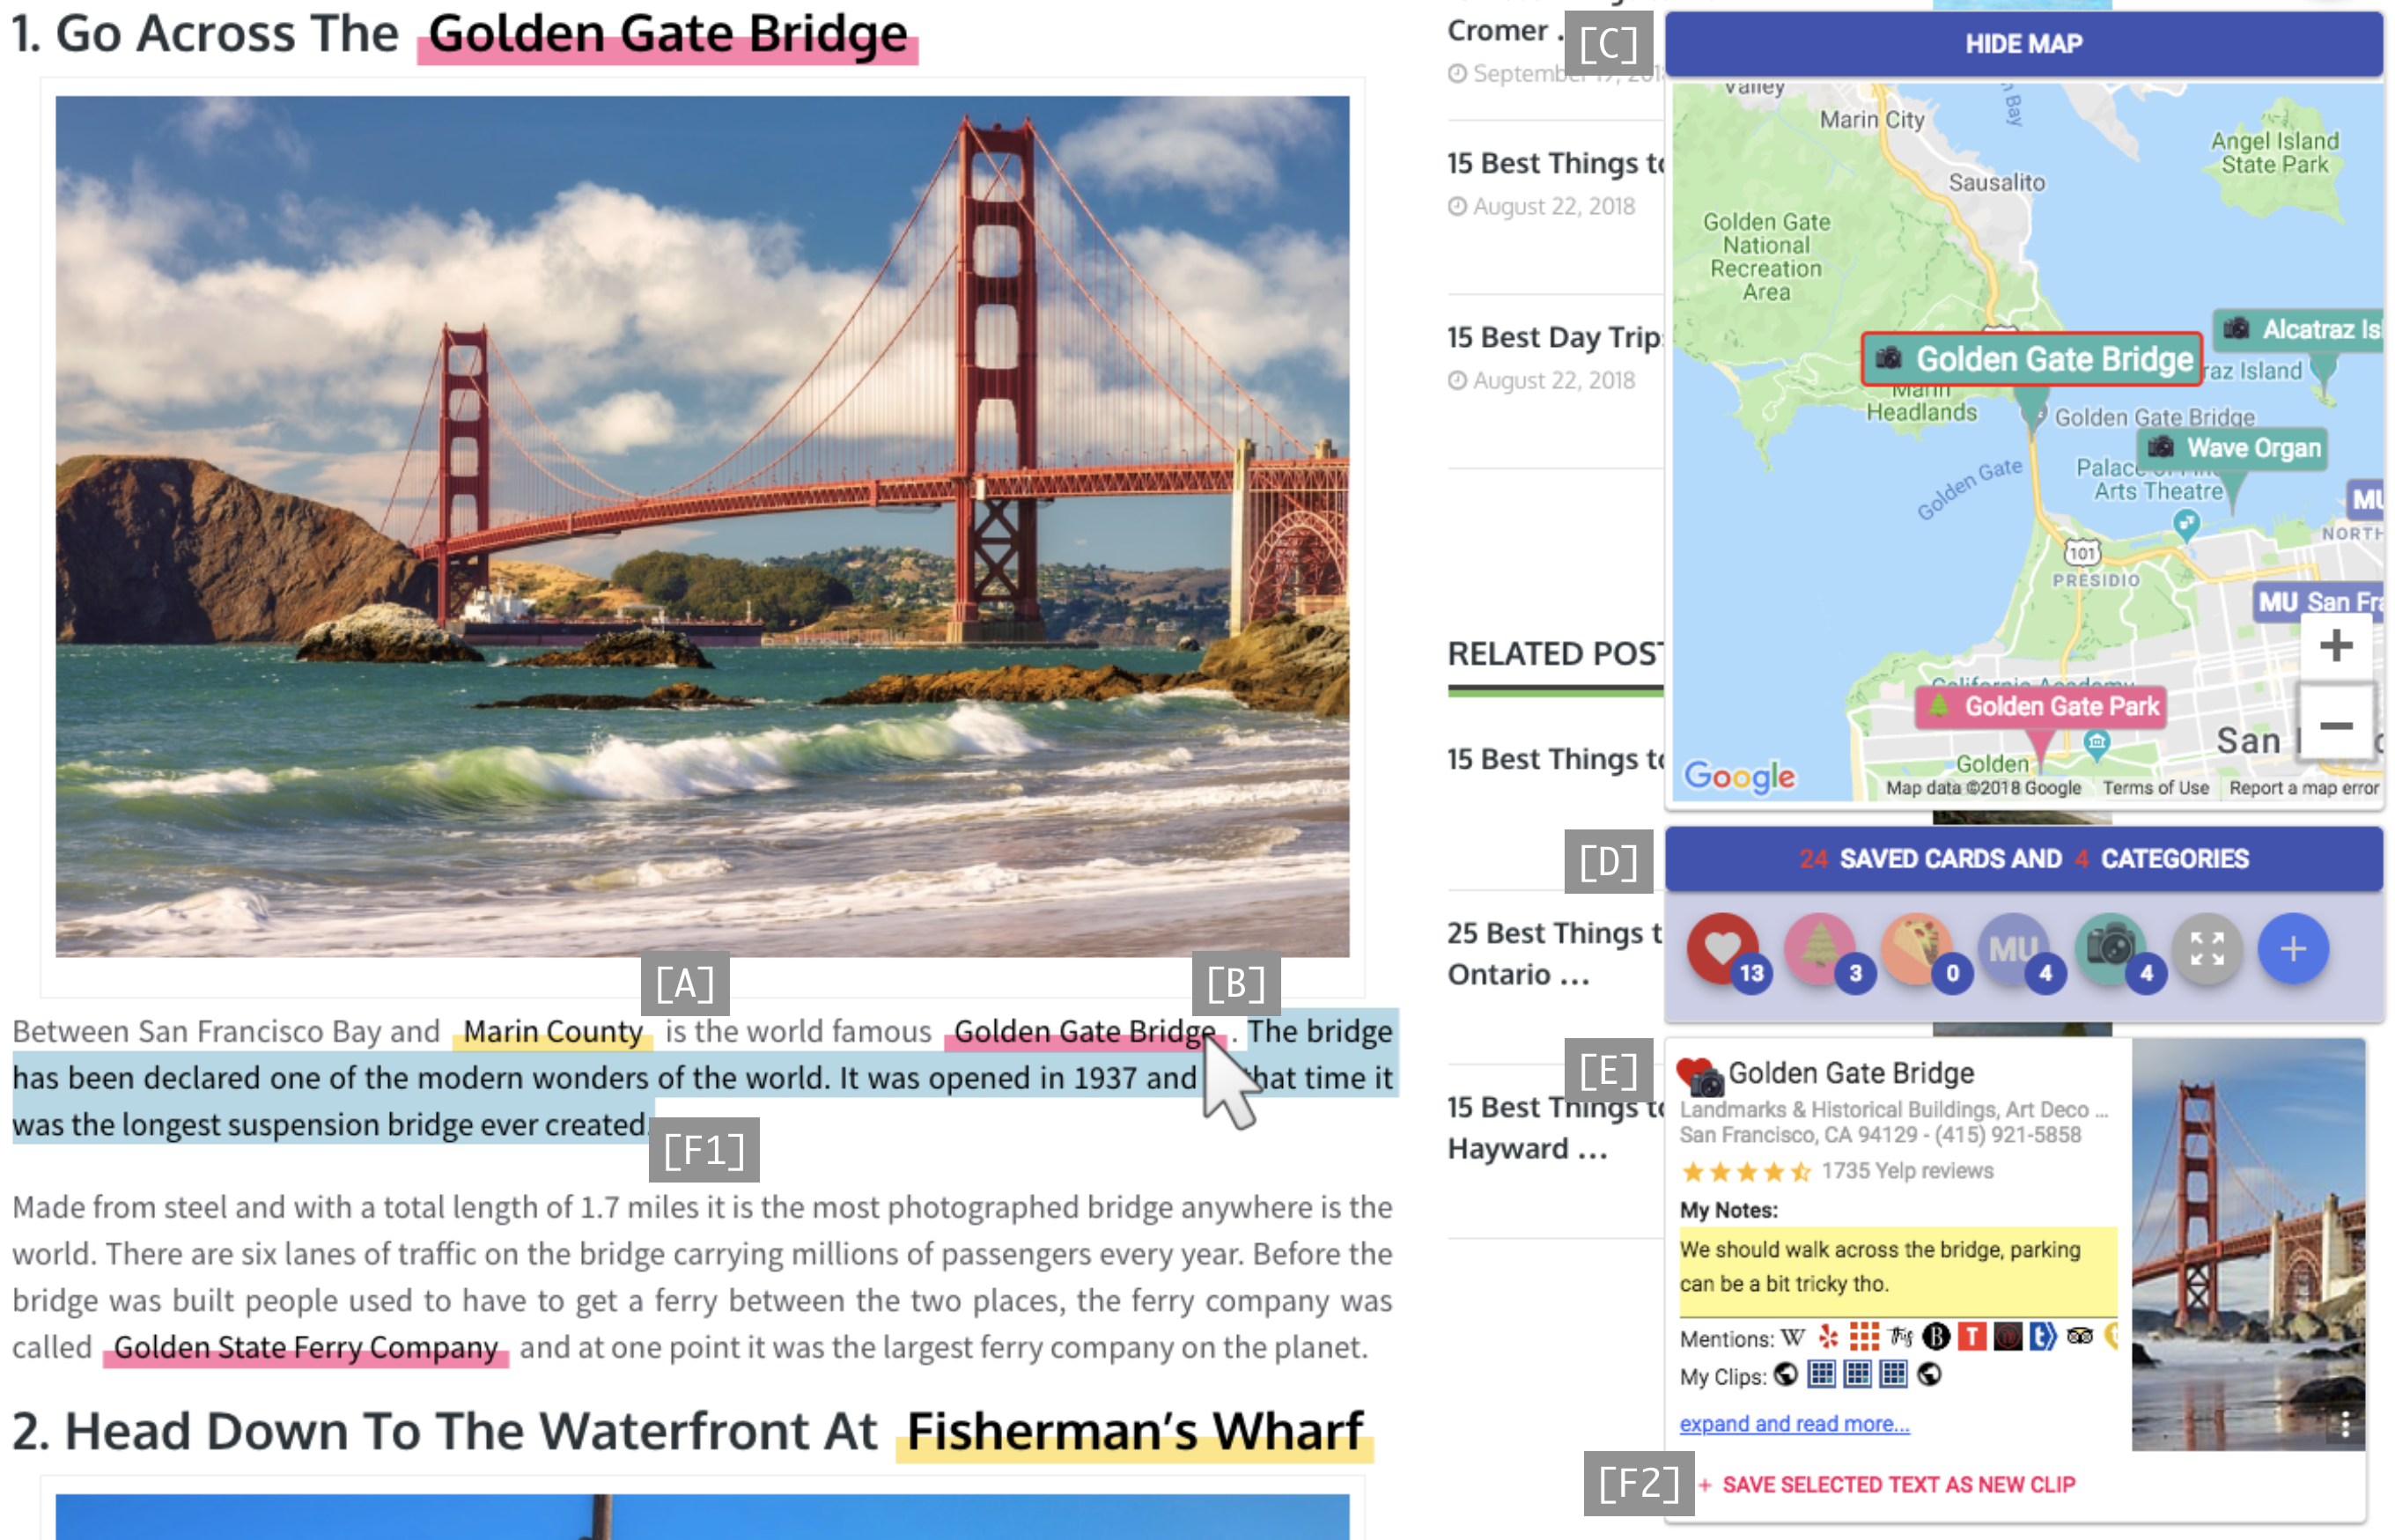
\includegraphics[width=1\textwidth]{Chapters/Fusion2/main3.png}}
    \caption[An overview of the Fusion browser add-on.]{An overview of the Fusion browser add-on. Fusion identifies and highlights entity mentions on webpages [A,B] to indicate additional information is available. Highlights in red [B] indicates users had previously interact with the entity. Hovering an mention [B] brings out its corresponding entity card [E] as an overlay, with relevant information ``infused'' from other pages and knowledge bases as \emph{mentions}. Users can also save notes or selected sentences [F1] to a card as \emph{clips} [F2]. Saved clips are then automatically ``diffused'' to other webpages that mentioned the same entity. Users can also create categories [D] and drag the card under them. Finally, the Map view [C] shows its location in context of previously saved entities.}
    \label{fig:main_fusion}
\end{figure}


Whether planning a trip to a new city, figuring out which camera to purchase, or researching the different treatments for a medical issue, learning and searching for information online has become the most common way that people make sense of the world today \cite{mar2006exp,pirolli1999information}. People spend a significant amount of time exploring available options and gathering evidence about them that are scattered across multiple webpages in order to make informed decisions.  Estimates suggest that up to 33\% of the time spent online, or, as of 2009, more than 24 billion hours per year in the US alone, are spent doing this type of aggregation and synthesis \cite{mar2006exp,kellar2007field,rose2004understanding,forrester}. Consider for example the task of planning a trip: there may be hundreds of possible restaurants to dine at, attractions to see, and places to stay, each with corresponding evidence about its suitability for an individual's goals and preferences. Evidence about each of these options is often spread out across multiple search results, such as Yelp or TripAdvisor reviews, top ten lists, travel blogs, forum posts, and travel guides. These webpages typically contain sets of overlapping options along with subjective evidence and past experiences about them. In order to compare different options, users need to go through a large number of webpages and cross-reference between them to synthesize evidence about each potential option.  However, this process of intense cross-referencing and note taking for sensemaking across webpages can be disruptive during reading and consuming information \cite{o1996towards,marshall1999introducing,tashman2011liquidtext,bianchi2015designing}, and is poorly supported by current browser and note taking interfaces. As the amount of user-generated content on the internet grows, supporting users in fully benefiting from this large repository of rich evidence is likely to become increasingly important \cite{mudambi2010research,gan2012helpfulness}.

Due to the ubiquity of entity-related web queries in online sensemaking tasks \cite{guo2009named,lin2012active}, one way that search systems have tried to support the above process has been by focusing on entity-centric approaches that present information about relevant entities in the search interfaces. For example, entity cards with rich attributes for entity-bearing search queries \cite{miliaraki2015selena,bota}, lists of important entities to be used as subsequent queries (such as listing actors when searching about a movie) \cite{blanco2013entity,bordino2013penguins,klouche2015designing}, or factual attributes about an entity or relationships between entities (such as the population of a city) \cite{balog2010overview,cheng2007entityrank,D15-1038}. While these approaches can efficiently provide factual and structured information about entities in search interfaces  (such as figuring out the location of a restaurant), in many cases people still depend on examining and synthesizing the unstructured and descriptive information scattered across multiple webpages opened in their browsers. This is especially true when comparing and making decisions about many entities in a complex task (such as making an expensive purchase). In these cases, there is no single objective answer that can be surfaced in a search results page directly. 

Although most prior work on entities have focused on providing objective information focused around a single entity during retrieval \cite{miliaraki2015selena,bota}, we posit that entities can also be useful for more complex exploratory search tasks by acting as a substrate connecting different information sources and the user's mental model. Leveraging them has the potential to enable deeper interactions with unstructured online information by focusing on meaningful concepts rather than webpages. Furthermore, recent advances in entity linking algorithms have been particularly promising in bringing the ability to better understand web content to the browser interfaces where users read and learn from individual webpages. For example, leveraging common entities mentioned across webpages to provide a sensemaking structure for users conducting complex exploratory searches and foraging across multiple webpages.

In this paper, we explore a new paradigm for interacting with unstructured and potentially subjective evidence about entities while reading and foraging from webpages in an exploratory search task. Since the user's personal evaluation of subjective information and how it meets their goal is critical in this situation, our design goal was to help the user to see scattered evidence about an entity in one place while also attaching personal notes and web clippings. These together served as a way to build up an external mental model and track search progress.

To investigate our entity-centric approach, we developed a prototype browser add-on called Fusion. Fusion allows users to keep track of the information scattered across multiple sources by ``infusing'' evidence about an entity from other webpages to the webpage the user is currently reading. It also ``diffuses'' users' thoughts about different entities across webpages where the same entities are mentioned for future reference and to accumulate more evidence. In our user study, we tested how participants utilized our entity-centric approaches while conducting complex exploratory search tasks, focusing on whether Fusion allowed them explore, gather, reuse, and accumulate evidence about entity options across multiple webpages. The primary domain on which we aimed to test Fusion was a travel planning task with 20 participants. In addition, we also tested a camera shopping task with 8 participants who had varying domain knowledge.
%We investigate in a user study how this functionality supports users in exploring how different information sources described newly encountered entities, and is useful in externalizing their thoughts about entities which can be easily resurfaced on the interface whenever they encounter the same entities on different webpages.
Finally, we discussed implications for the design of future intelligent interfaces that can better understand the information being consumed by its users by taking advantage of advances in natural language processing to support online sensemaking in various scenarios.




\section{Related Work}

Past research has proposed a variety of approaches to better support complex search tasks at varying stages. Our work builds on this diverse literature by leveraging state-of-the-art entity-centric approaches in information retrieval and natural language processing to drive our infusion- and diffusion-based user interactions in an in situ interface. This allowed us to empower the browser interface to better understand the information being consumed by its users, and to provide an entity-centric approach to sensemaking and information foraging across multiple webpages.

\subsection{Saving and Organizing Information from the Web}

When reading individual webpages, users conducting exploratory search tasks often need to take notes or save information from many webpages \cite{mar2006exp}. Past work showed that up to 86\% of users save information from webpages when conducting search tasks \cite{lee2012survey}. Due to its ubiquity, browser add-ons supporting online foraging and organizing information have become popular and widespread in recent years, including Evernote with over 200 million users and Pocket with over 2 billion items saved. Researchers have also built tools to support online foraging from saving and organizing entire webpages \cite{card1996webbook} to specifying and saving parts of webpages and organizing them \cite{dontcheva2006collecting, sugiura1998internet,zhu2002hunter,chang2016supporting}. Extracting and saving information across webpages in an exploratory search task can be challenging in that these webpages typically contain evidence for overlapping options, but the majority of the information is unstructured, requiring users to manually cross-reference between pages in order to gather evidence about the same option. At the same time, prior work has also pointed to how frequent context switching between different documents and taking notes is distracting, and sometimes prohibits users from investigating deeper or stop to take notes in order to avoid disrupting the flow of reading \cite{o1996towards,marshall1999introducing,tashman2011liquidtext,bianchi2015designing}. One approach requiring content publishers to provide machine readable annotations such as using semantic web markups \cite{berners2001publishing,berners2001weaving}, has failed to gain momentum due to a lack of available end-user tools that can consume these annotations \cite{whatwentwrong}. Alternatively, researchers have also explored using in situ interfaces (e.g., a sidebar) to enable access to user notes while reading \cite{tashman2011liquidtext,notetoself}. However, past systems either persisted notes only on individual pages and do not support synthesizing across sources, or did not provide a scalable way for reusing and organizing large collections of saved notes.  In particular, \cite{notetoself} reported that their participants relied on skimming or targeted search using keywords from memory for re-finding previously saved notes, which potentially led to a large portion of user notes rarely re-accessed nor deleted. Fundamentally, note taking softwares treat options mentioned on webpages and users' notes about them as independent, and the cost of cross-referencing between webpages and their notes to accumulate evidence for the same options can be prohibitively high.

Another thread of research related to our work focused on saving entity information listed on webpages in plain text via end-user programming or interaction techniques. For example, \cite{bier2006entity} and \cite{stylos2004citrine} allowed for efficient copying and pasting of entity attributes  (e.g., addresses and phone numbers) by automatically identifying them in text, and \cite{thresher,huynh2005piggy,dontcheva2006collecting} assisted users in extracting both entities and their attributes from webpages (e.g., a list of faculty with contact information.)
While past work also points to users' needs to interact with entities and collect information about entities while browsing webpages, they mainly focused on helping users collect objective attributes about entities from individual pages and do not provide support for gathering descriptive and subjective evidence about entities across pages, which often play an important role in decision making during complex tasks such as trip planning. 

In this paper, we built a prototype browser add-on, Fusion, that aims to address the aforementioned limitations of prior work --- the high costs of reusing previously saved notes and evidence, cross-referencing, and context switching. Fusion utilizes open and commercial entity databases \cite{dbpedia} and state-of-the-art entity linking algorithms \cite{spotlight} to automatically identify entities mentioned across information sources in an exploratory search task. When a user encounters an entity on a webpage, Fusion presents an in situ entity card with rich attributes similar to ones used in modern commercial search interfaces \cite{miliaraki2015selena,bota}. For example, showing the location and review ratings of different restaurants mentioned on a webpage. The in situ entity cards also serve as a foraging structure where users can attach notes and web clips to them. This also allows Fusion to automatically resurface previously saved notes and clips on other webpages that also mention the same entities so previously saved information can be efficiently reused.

\subsection{Entities in Search Interfaces}

Users conducting exploratory search tasks are unsure about their goals, and often need to rely on reading and foraging from multiple webpages to iteratively learn about the available options and gather useful evidence \cite{mar2006exp}. Prior work on search engine interfaces have focused on ways to help searchers better orient themselves by providing an overview of webpages in a search result \cite{marchionini2000agileviews,patterson2001predicting,tretter2013searchpanel} or managing multiple searches and information sources \cite{morris2008searchbar,hahn2018bento}. More closely related to our work, significant research has also gone into entity-centric approaches due to the ubiquity of entities in online sensemaking tasks. Studies in 2009 and 2012 have found that entity-bearing queries and entity category queries accounted for up to 71\% to 85\% of web search traffic \cite{guo2009named,lin2012active}. This has led to significant academic and commercial efforts devoted to building large-scale entity databases (such as DBPedia \cite{dbpedia}, Yelp.com, and Google Places), and a decade of research on ways to enrich search interfaces with information about entities. Major threads of research include identifying entities mentioned in queries to present entity cards for quick referencing \cite{bota,miliaraki2015selena}, answering factual questions about entities directly \cite{D15-1038}, and showing lists of related entities to be used as subsequent queries \cite{blanco2013entity, bordino2013penguins,klouche2015designing}. 

While these approaches have made great strides in making retrieval more efficient based on better understandings of users' intent \cite{miliaraki2015selena} and the content of web documents \cite{fernandez2008semantic}, significant user effort is still required after retrieving documents --- when consuming and extracting information from individual webpages and organizing them. Yet the browser interface where users conduct these intense sensemaking and decision-making processes remain largely unchanged, and relatively less explored in research \cite{whatwentwrong}. Current browsers treat entity mentions and their evidence described in each opened webpage independent of other webpages, making it difficult for users to cross-reference, forage, and keep track of what they are interested in and why across webpages. In this paper, we instead utilize techniques used in search systems to explore an alternative design space where the browser is aware of the same entities mentioned across webpages opened during an exploratory search task. For this, we propose to empower the browser interface with readily available open and commercial entity databases \cite{dbpedia} and entity linking algorithms \cite{spotlight}, and explore entity-centric approaches for supporting sensemaking across webpages.


\begin{figure}
    \centering
    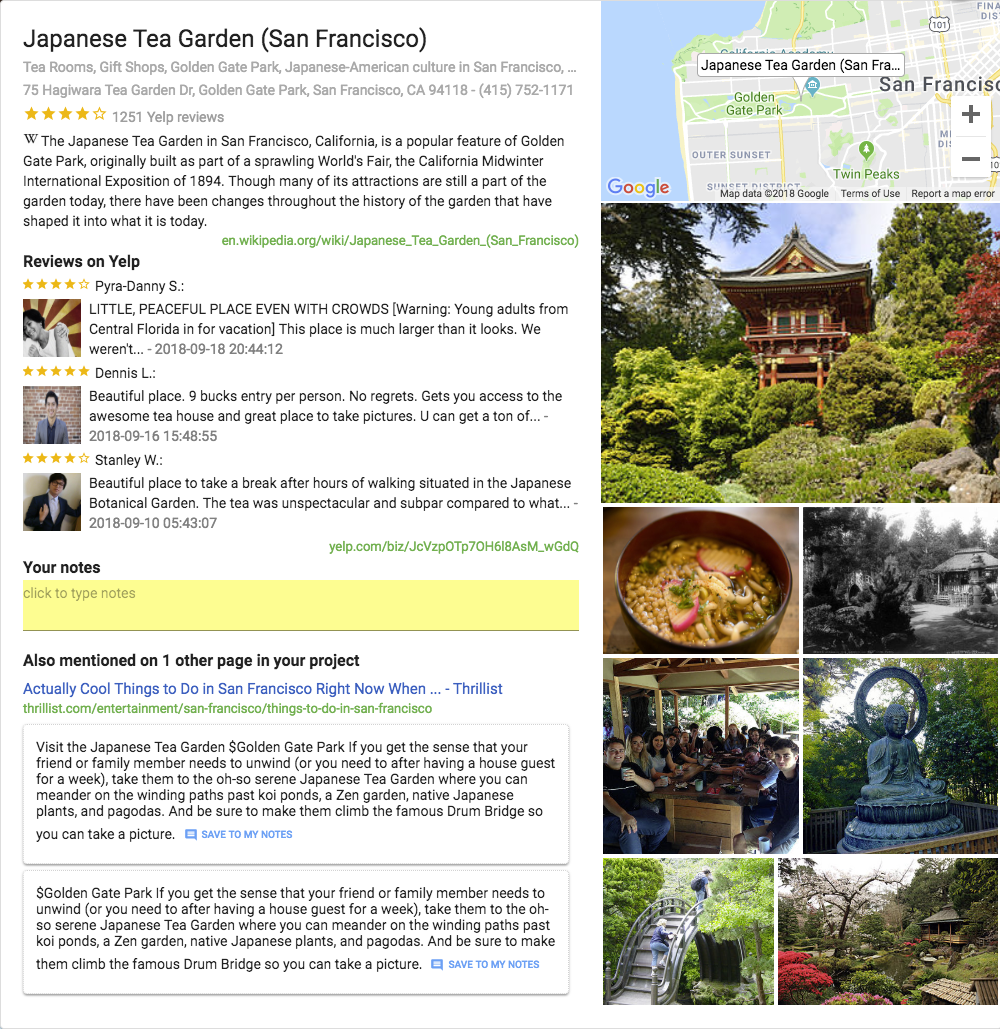
\includegraphics[width=1.0\columnwidth]{Chapters/Fusion2/expanded.png}
    \caption[Expanded view for an entity card.]{Expanded view for an entity card showing information \emph{infused} from external knowledge sources (Yelp and Wikipedia), user's notes, and evidence of the same entity from other webpages in the exploratory search task. See Figure~\ref{fig:main_fusion} for the non-expanded view of an entity card.}
    \label{fig:expanded_fusion}
\end{figure}


\section{System Design}
We introduce Fusion, a novel browser add-on that uses an entity-centric approach to facilitate sensemaking across webpages in exploratory search tasks. Figure \ref{fig:main_fusion} shows an overview of how an exploratory searcher planning a trip might use Fusion. Unlike previous approaches for supporting sensemaking in exploratory search tasks, such as re-ranking or enriching the search result lists or using external note management interfaces \cite{syed2017optimizing,miliaraki2015selena}, we focused on providing \emph{in situ} support for sensemaking while reading and capturing information.  Fusion provides users a lightweight overlay interface embedded and synced across webpages in different browser tabs, allowing users to make quick and lightweight cross-referencing without switching between tabs, windows, or applications. The two core components of Fusion augment content in two ways, which we introduce as ``\emph{infusion}'' and ``\emph{diffusion}.'' First, when users open a webpage from their search results, the system ``infuses'' the webpage with relevant snippets about mentioned entities from other webpages in their search results and external knowledge sources to help users cross-reference and evaluate newly encountered options. Second, when users save notes or extract content from a webpage, the system ``diffuses'' them to mentions of the same entities in other webpages of the same task, allowing them to easily access previously saved information without having to switch to and search through a separate interface \cite{notetoself}. To drive these operations and connect the different webpages, we use the DBpedia Spotlight algorithm \cite{spotlight} to automatically identify common entities mentioned in the different webpages. In our implementation, we use Yelp and DBpedia as our entity repositories and focus on travel planning tasks, but other knowledge bases can also be used or added to support other types of projects. For example, using the Microsoft Academic Graph\footnote{https://www.microsoft.com/en-us/research/project/microsoft-academic-graph/} and the Gene Ontology \cite{gene} as knowledge bases to support literature review projects in biology. In the next subsections, we will first describe in detail how Fusion identifies entities in web content, and then describe both the infusion- and diffusion-based features.


\begin{figure}
    \centering
    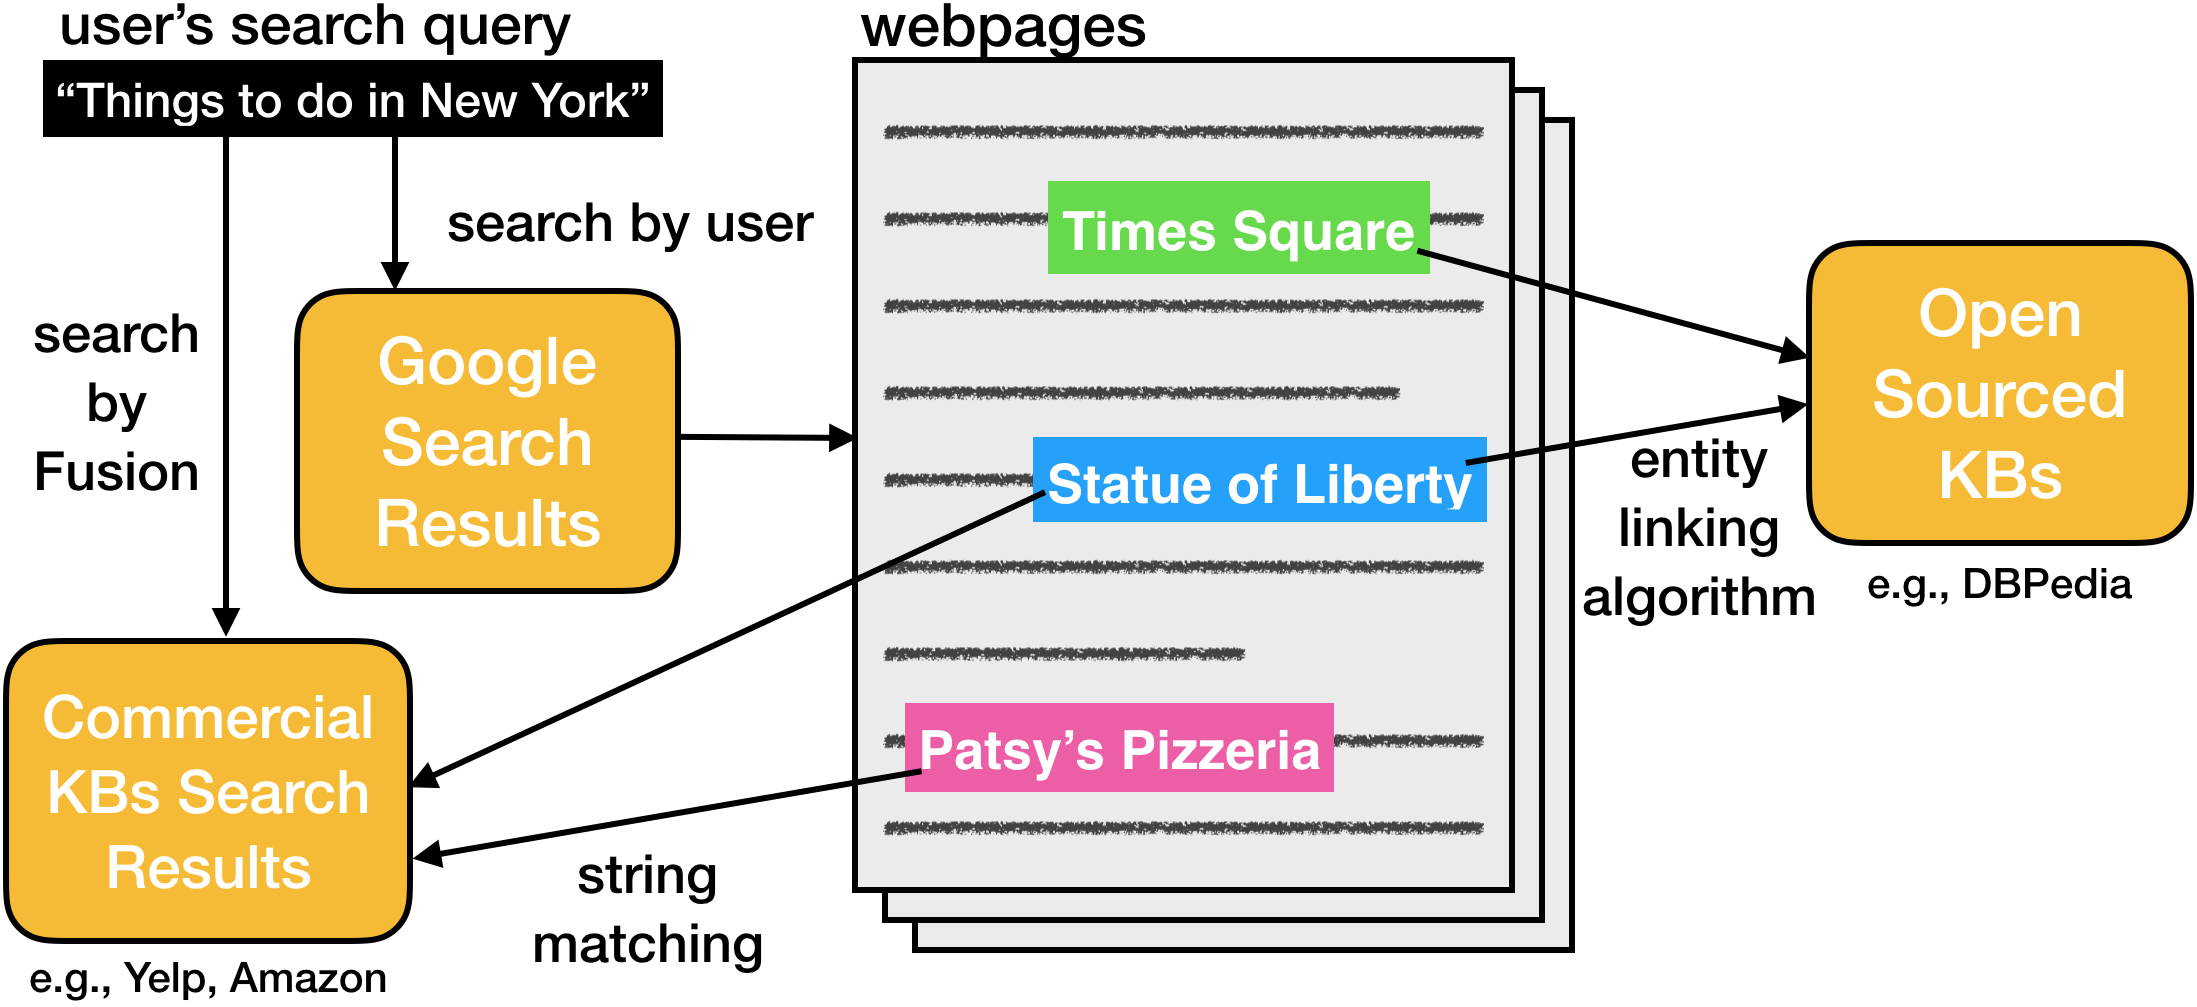
\includegraphics[width=0.5\columnwidth]{Chapters/Fusion2/entity_linking.png}
    \caption[Linking entities from webpages to open and commercial knowledge bases.]{Fusion links entity mentions from webpages to both open and commercial knowledge bases.}
    \label{fig:entity_linking_fusion}
\end{figure}

\subsection{Linking to Open and Commercial Knowledge Bases}
Users can add searches and individual webpages to their Fusion projects. When a search is added to a Fusion project, Fusion parses the HTML of the search results page to obtain the list of webpages. In the background, Fusion analyzes the content of webpages to identify entities mentioned using the following methods (Figure~\ref{fig:entity_linking_fusion}). First, it uses the Spotlight library \cite{spotlight} to identify entities mentioned in different surface forms (e.g., San Francisco Museum of Modern Art and SFMoMA) to DBpedia which contain rich attributes extracted from Wikipedia. Unlike DBpedia, Yelp is a commercial services in which neither the entity database nor a pre-trained entity linking model were publically available. In order to identify Yelp entities in webpages, we use keywords and a location extracted from the original query term users performed on Google (e.g., best sushi bars in new york) to query the Yelp Search API\footnote{https://www.yelp.com/fusion} for a list of 450 Yelp entities. This allows Fusion to retrieve from closed databases for entities that match with users query intent and information needs. Simple string matching is used to identify mentions of any Yelp entities on each webpage.

To avoid showing duplicate entities from DBpedia and Yelp and to improve the coverage of identifying Yelp entities, Fusion use a location-based heuristic to merge entities from the two sources: two entities are merged if 1) they are from different knowledge bases, 2) have overlapping surface forms listed in the knowledge bases, and 3) have geographic coordinates that are less than two kilometers from each other. Using simple string matching to identify Yelp entities on webpages can have limited coverage since Yelp only lists one surface form for each entity (e.g., name of restaurant). However, if a Yelp entity was merged with a DBpedia entity, it is automatically applied to mentions of different surface forms as identified by the entity linking algorithm \cite{spotlight}.

A caveat of driving end-user interfaces with machine learning is potentially having the model make occasional mistakes that can degrade the user experience, and it is crucial to provide mechanisms for the users to recover from them \cite{lewis1995designing,lee2010gracefully,kocielnik2019will}. For example, in a trip planning task, a webpage might miss a popular destination not recognized by the Spotlight algorithm, not listed on DBpedia, or not covered in the results returned from the Yelp API. In addition, since Fusion depends on users' original search terms to obtain relevant entities via the Yelp Search API, webpages opened by typing URLs into the address bar does not support recognizing Yelp entities automatically in the current implementation. These issues may disrupt users' exploration processes, forcing users to resort to external tools for capturing information. To provide a way to recover from these situations, Fusion allows users to manually mark phrases on the webpage as entities and link them to entities in DBpedia and/or Yelp (Figure \ref{fig:custom_fusion}, we will describe in detail in the next subsection.) Finally, Fusion extracts the paragraphs around entity mentions from each webpage as supporting evidence.

\subsection{Infusion: Gathering Evidence from other Webpages}

A common activity in complex exploratory search involves collecting information from multiple sources and make informed decisions.
%Our preliminary survey, as described in the Introduction, showed that 88\% of participants ``use information from multiple webpages to verify uncertain information.'' % removed from intro
%echoed by our preliminary study described in the Introduction in which 88\% of participants reported that they typically gather evidence from multiple sources ``in order to verify uncertain information.'' %Similarly, 83\% reported that they would typically perform at least 4 searches to gather information when planning a trip, and 50\% would spent at least 4 hours searching when purchasing something important or expensive.
Fusion supports this need by ``infusing'' entities mentioned on a page with context pulled from other webpages mentioning the same entity or entries in external knowledge sources (in our current implementation, DBpedia and Yelp). When users open a webpage, entity mentions that were recognized by Fusion are highlighted with a half-height yellow highlight (Figure \ref{fig:main_fusion}, A) to indicate they have information from other sources. By hovering over an entity, a user can see an ``entity card'' (Figure \ref{fig:main_fusion}, E) which displays those sources and relevant information (e.g., number of stars on Yelp, paragraphs from other web sites in which the entity was mentioned) which a user can use to gain context about the entity beyond the current webpage \cite{bota}. To read the mentions, the user can click on the icon of each external source to see an extracted snippet. Alternatively, the user can also expand the Card to see a larger view (Figure~\ref{fig:expanded_fusion}), showing all mentions, multiple images, and a map of the location using metadata from Yelp and/or DBpedia. 

As a running example, a user planning a trip to a new city might open an article from a travel blog and see all the destination and restaurant mentions highlighted in yellow by Fusion. As the user reads the article, he or she finds a highlighted restaurant and the author recommended it for reasons that also fit our user's personal interests. However, instead of relying on this single piece of evidence, the user hovers over the restaurant name to query for its entity card for additional information. The entity card contains Yelp review scores, Wikipedia description, and a list of relevant snippets from other webpages from the user's previous searches. After reviewing these information, the user drags the entity card under the restaurant category created previously. 

While the state of entity recognition is continuously improving, there are situations when an entity isn't recognized, for example due to a lack of coverage in the recognition system or errors on the page itself. To recover from cases where an entity of interest was not recognized by Fusion, the user can still create a custom entity card by first selecting the entity name on the webpage, and click on the ``Create Card'' button in Fusion (Figure \ref{fig:custom_fusion}). In the background, Fusion queries the two knowledge sources for candidates, merges the two results lists using the location-based heuristics described in the previous subsection, and finally presents the list of candidates from which the user can pick.  Alternatively, if the entity was not found in the knowledge bases, the user can still create a custom entity card (Figure \ref{fig:custom_fusion}). In early pilot testing, we found a common user need for this in creating an ``ad hoc'' entity where there might not be a specific, concrete location or entity (e.g., creating a card to collect tips about packing for Machu Pichu or general descriptions of beaches in New England). 

There are several ways in which entity cards might be surfaced to provide context to users. In the first version of Fusion, we detected which entities were mentioned in the browser viewport and displayed a list of entity cards. Our intention in exploring this design was to provide a visual trigger for users to learn about the context of entities and potentially act on that context by annotating or saving relevant entities. However, participants in our preliminary user studies raised the issue that many of the entities surfaced were not relevant to their tasks, and having to sift through the list of entity cards and locate relevant entities was time consuming. Many of these irrelevant entities were either overly general locations (e.g., U.S.A), ambiguous or partial matches (e.g., ``park''), or general knowledge entities from Wikipedia (e.g., Cuisine of the Southern United States). While it is possible that approaches taking into account the user's prior knowledge about the task and their query intent might improve the relevance of returned results (e.g., \cite{pasupat2014zero}), the density of entities within the browser viewport constitutes a more fundamental issue that leads to cluttering the browser interface and overwhelming users with too much information at once \cite{wilson2008improving}. Based on these observations, we changed the interface from actively pushing all the entity information to the users to underlying recognized entities and allowing users to query information for entities that they determined to be relevant.

\begin{figure}
    \centering
    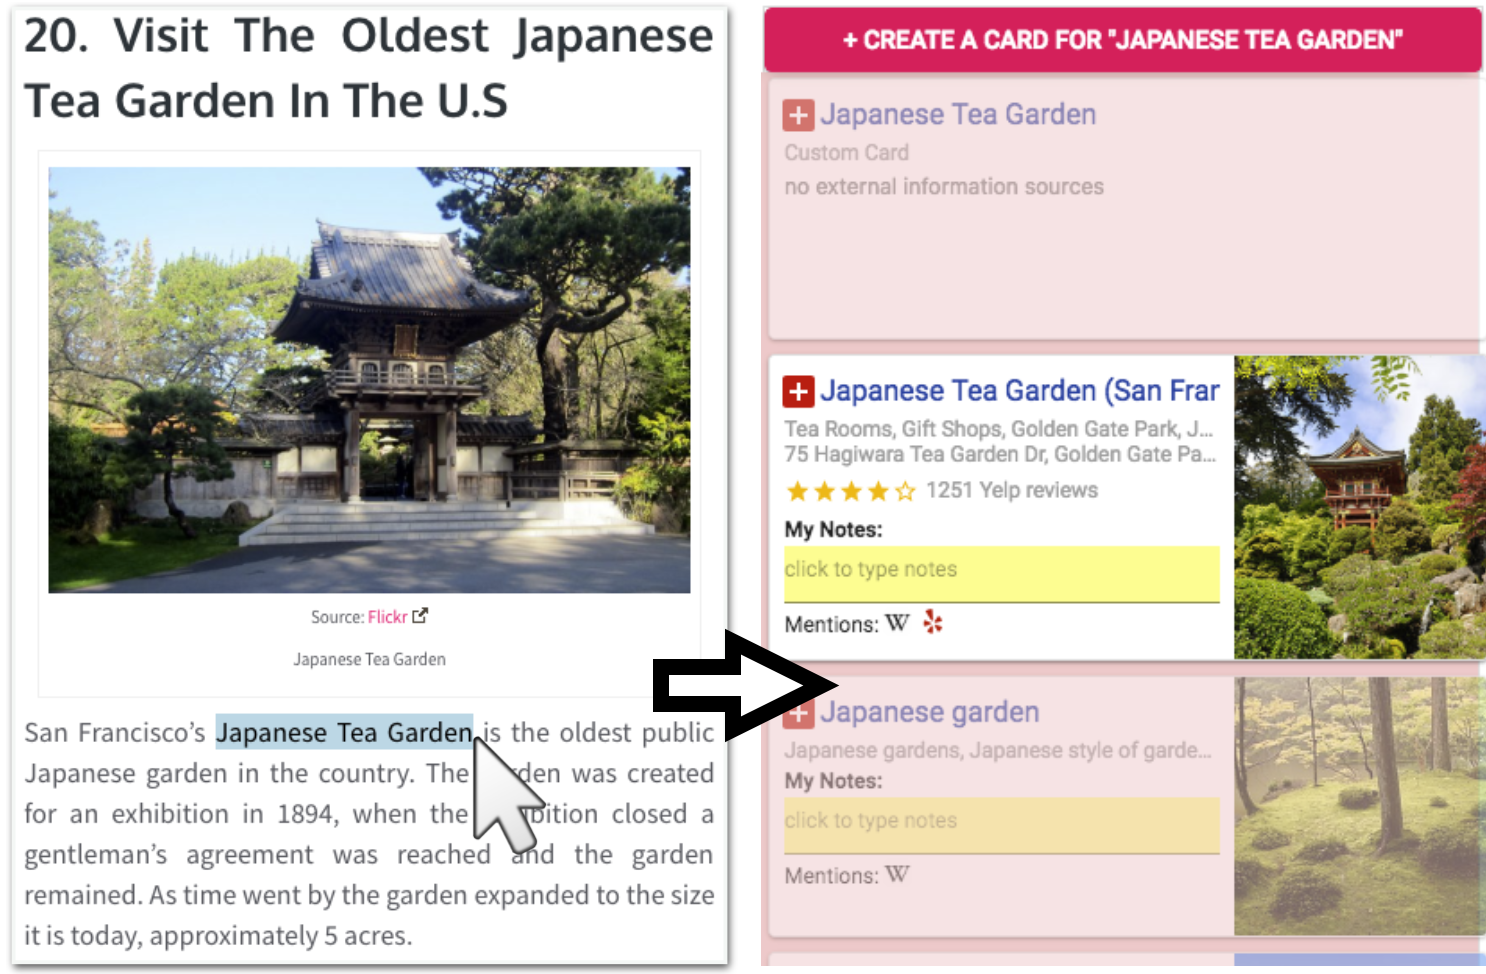
\includegraphics[width=0.5\columnwidth]{Chapters/Fusion2/custom4.png}
    \caption[Creating manual entity cards.]{To create a missing entity, users can select a phrase (here, Japanese Tea Garden) on the page and see a list of candidates to choose from. In this case, the top 3 candidates were 1) a Custom Card not linked to external knowledge bases, 2) an entity card linked to a specific Japanese garden on both Yelp and DBpedia, and 3) and entity card linked to the general entity for Japanese gardens in DBpedia.}
    \label{fig:custom_fusion}
\end{figure}


\subsection{Diffusion: Propagating Notes to other Webpages}

After using ``infused'' context to judge the relevance and suitability of options (i.e., entities), users often need to keep track of and organize the options they found valuable. At the same time, users may evaluate newly encountered options against ones they have already saved. Typically, this happens by copy-pasting or typing entity names and notes into a separate interface, for example a separate document or email or note taking software (e.g., Evernote). Researchers have tried to lower the switching cost involved in this interaction \cite{o1996towards,tashman2011liquidtext}, for example, by adding a sidebar to the browser for taking free-form notes \cite{notetoself}. However, in the cases when the user encounters additional evidence about an option they already have information about, they need to re-find it in the external system before being able to continue, which can lead to significant adoption issues \cite{notetoself}.

Fusion addresses this challenge this by ``diffusing'' notes that users associate with an entity to all other webpages in the project that also mentioned the same entity, reducing the need for user-driven re-finding. Continuing with our running example of trip planning from the previous subsection, imagine that after the user reviewes the information in the restaurant entity card, he or she decides to take notes and save the restaurant for future reference. To do so, the user can add various levels of annotation to the card, including just ``hearting'' it to save it in the Saved Cards view as uncategorized  (Figure \ref{fig:main_fusion}, top-left corner of E), typing notes about reasons for saving it (Figure \ref{fig:main_fusion}, yellow region in E), or selecting sentences (Figure \ref{fig:main_fusion}, around B) from the webpage to add to the entity card as a clip (Figure \ref{fig:main_fusion}, E). When the user moves on to other webpages in the project, mentions of the same restaurant will be highlighted in half-height light red (Figure \ref{fig:main_fusion}, B), indicating that the user previously interacted with this entity, and upon hovering will see its entity card with annotations and clips they have previously added. 

Using this entity-centric approach, users can save notes of information collected across webpages under entity cards without having to switch back and forth between the browser and note-taking software, and easily re-find and reuse previously saved information when encountering the same entities on other webpages. To recover from cases where an entity of interest was not recognized by Fusion automatically, users can manually create entity cards using interactions as described in the previous subsection. If a user created an entity card that was linked to DBpedia and/or Yelp entities, all the information that was associated with them will also appear on the user-created entity card. This ensures that users can still save and retrieve information to accumulate what they have learned, even when an entity mention was not automatically recognized by Fusion.

\subsection{Project Overview and Organizing Entities}

\begin{figure}
    \centering
    \frame{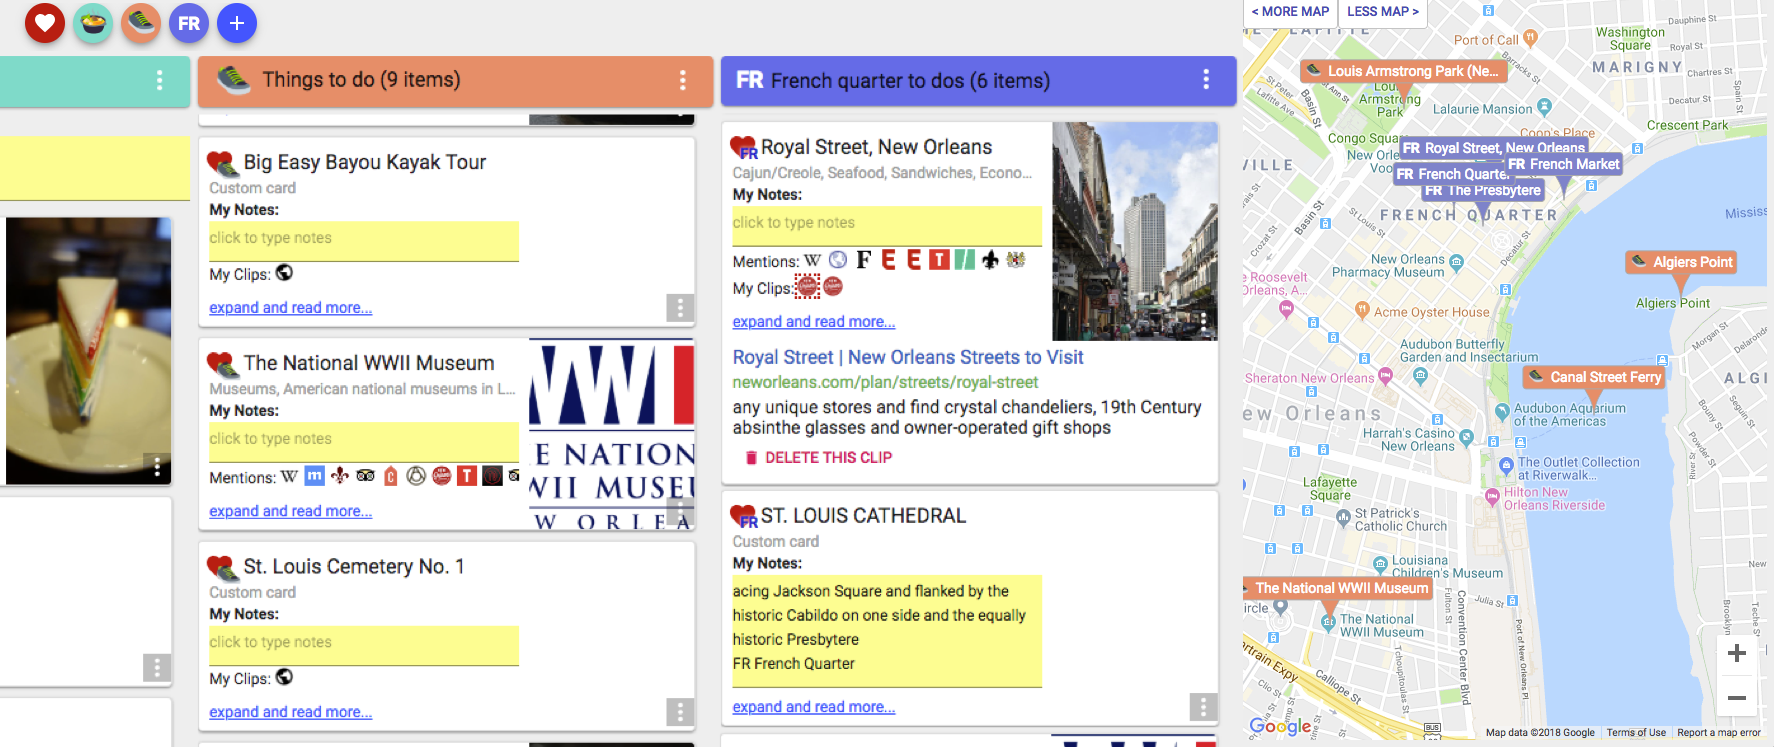
\includegraphics[width=1\textwidth]{Chapters/Fusion2/project2.png}}
    \caption[An project overview page created by one participant.]{An project overview page created by one participant after searching for 50 minutes, containing entities saved under different categories, text clips from multiple webpages, and typed notes. Custom cards were created, including one for a kayaking tour that was not available on Yelp and DBpedia. The entity cards were scaled for clarity in this figure.}
    \label{fig:project_fusion}
\end{figure}


As users in exploratory search tasks gradually progress from discovering entities and gathering evidence to focus more on synthesizing and making decisions, they may also need to organize and compare the collected entities. For example, in a travel planning task, users may want to group their entities into categories of restaurants, attractions, and hotels for comparison, and also to figure out the location and distances between the different entities to plan their trips.

In Fusion, in addition to simply ``hearting'' an entity card, users can also create categories with custom names, colors, and icons in the Saved Cards view (Figure \ref{fig:main_fusion}, D). To categorize an entity card, simply drag and drop it between categories. This allows users to start structuring any time during their exploratory search process when the need arises. Saved geographic entities (entities with coordinates metadata from Yelp and/or DBpedia) will also show up in the Map View  (Figure \ref{fig:main_fusion}, C) with their icons and color coded pins. In addition, when users hover over an unsaved geographic entity on the current webpage, its location is also shown on the Map view. This allows users to better situate a newly encountered option with previously discovered entities to make informed decisions. For example, a user could quickly figure out that a hotel recommendation on the current webpage is not relevant by noticing in the Map view that it is too far away from most attractions that they have saved previously from other webpages. At later stages of the exploration process, users might shift their focus from reading and gathering information to synthesizing and organizing information. For this, they can open the Project Overview page by clicking on the expand button in the Saved Cards view to see all their entity cards listed in multiple columns of each category along with an integrated map view (Figure \ref{fig:project_fusion}).

\subsection{Implementation}

Fusion was built as a add-on for the Google Chrome browser implemented in Javascript using the ReactJS library. The application uses Google's Firestore real-time database to store mappings between webpages and entities and user-generated notes and clips. We utilize the Yelp Search API to fetch entities from Yelp, and we use the open-sourced DBpedia Spotlight \cite{spotlight} software in a custom backend that identifies DBpedia entities \cite{dbpedia} in webpages and syncs them with the end-user interface through Google's Firestore service.

\section{Evaluation}
We conducted a lab study to evaluate the benefits of Fusion for users conducting complex exploratory search tasks. The main goal of our study was to explore the benefits and challenges of an entity-centric approach for reading, cross-referencing, and collecting information across multiple webpages in the browser. More specifically, we explored whether participants find our entity-centric approach to be beneficial for sensemaking across webpages during a complex exploratory search task. 

\subsection{Study Design}
We recruited 20 participants (age=19-43, $\bar{x}$=25.40, $\sigma$=7.67, 55\% female) from a local participant pool. The study began with a pre-survey to collect demographic information and self-reported expertise in the domain of the assigned tasks (described below). The main part of the study was to conduct an exploratory search for 50 minutes using Fusion, followed by a 30 minute post-survey about the experience. The study was conducted using 12.5 inch Chromebooks running Chrome version 69. Each participant was compensated 15 USD. 

The primary domain on which we aimed to test Fusion was a travel planning task with the following description:

    \begin{tightquote}
You and your friends are going on a trip to New Orleans. Help the group figure out which places you should go and where to eat during the trip. 
    \end{tightquote}

\noindent This travel planning task was designed to test Fusion's ability to support collecting and managing evidence from multiple sources for multiple options. Travel planning has a number of characteristics that make it a good task to test new sensemaking and exploratory search approaches. For example, information is often scattered across many sources; there is a strong degree of contextualization and personalization needed (e.g., traveling somewhere with kids is very different than without); and evidence such as reviews can be noisy and subjective \cite{zhang2012human,chen2015tripplanner}.  This domain also worked well with the backing knowledge bases in our implementation -- Yelp provided entities for local restaurants and tourist attractions with images and reviews, while DBpedia provided general entities extracted from Wikipedia. We tested Fusion using the travel planning task with 12 randomly selected participants. 

In addition to our primary domain, we also used a camera shopping task with 8 participants using the following description:

\begin{tightquote}
A friend is asking for your help to figure out what DSLR and mirrorless cameras are and which model she should buy as a beginner.
\end{tightquote}

\noindent This camera shopping task aimed to test the boundary conditions of Fusion. Unlike the travel planning task, Fusion's current implementation does not have a knowledge base specialized for camera products, and most webpages in this task do not contain any geographic entities. However, unlike the travel task which assumes only general knowledge, camera shopping for DSLR or mirrorless cameras involves significant learning and necessary expertise with concepts and terms that might be unfamiliar. Participants who were novices in the domain would need to first learn the technical terms and domain knowledge in cameras and photography before advancing to the stage where they can evaluate different options (i.e., camera models) to collect evidence. In theory, Fusion could also help with general knowledge-building using information from DBpedia. For example, helping novice participants to understand and take notes about unfamiliar technical terms (e.g., full-frame CMOS sensors) using entity cards from DBpedia. We chose these characteristics to probe the application of an entity-centric approach in a situation where there might not be good coverage of entities and attributes, and where some users might not have the required domain knowledge to evaluate the different options in webpages. 

In both tasks, we used the following description as a motivator to encourage the participants to put in more research effort, derived from previous studies of sensemaking:

\begin{tightquote}
Imagine after this task you will share your project overview page with your friend(s), along with a short summarization in an email. To convince your friend(s) of your choices, provide enough reasons and information about your choices.
\end{tightquote}

\noindent After conducting the main task for 50 minutes, participants spent another 30 minutes answering a post-survey using both Likert-scale ratings and free-form responses focused on their experiences during the main task and to compare Fusion with their current practices.


\subsection{Results}

\begin{table}
  \centering
  \footnotesize
% question, \#of sources, \#of clips, \#of turkers
  \begin{tabular}{ r  r l   r l r l }
  
	
	\multicolumn{1}{p{0.4\columnwidth}}{Statement (7-point Likert-scale responses)} &
	\multicolumn{2}{c}{Travel} &
	\multicolumn{2}{c}{Camera (experts)} &
	\multicolumn{2}{c}{Camera (novices)} \\
    
	\hline
	
	
%	P1 &
	\multicolumn{1}{p{0.4\columnwidth}}{Presurvey: \textit{I know what DSLR cameras are}} &
	\multicolumn{2}{c}{-} &
    6.75 & $\sigma$=0.50 &
    3.50 & $\sigma$=1.73 \\
    
%    Q1 &
	\multicolumn{1}{p{0.4\columnwidth}}{\textit{It is an improvement to my current practice}} & 
    5.67  & $\sigma$=1.11 &
    5.75 & $\sigma$=0.50 &
    2.75 & $\sigma$=2.22 \\
    
%    I1 &
	\multicolumn{1}{p{0.4\columnwidth}}{\textit{The cards were useful for reading new pages \& learning new thing}s} &
    5.42 & $\sigma$=1.11 &
    6.00 & $\sigma$=0.82 &
    3.25 & $\sigma$=2.63 \\
    
%    I2 &
	\multicolumn{1}{p{0.4\columnwidth}}{\textit{Information from Yelp was useful
}} &
    5.92 & $\sigma$=0.86 &
	\multicolumn{2}{c}{-} &
	\multicolumn{2}{c}{-} \\
    
%    I3 &
	\multicolumn{1}{p{0.4\columnwidth}}{\textit{Information from Wikipedia was useful}} &
    5.67 & $\sigma$=0.85 &
    5.50 & $\sigma$=1.29 &
    4.00 & $\sigma$=2.45 \\
    
%    I4 &
	\multicolumn{1}{p{0.4\columnwidth}}{\textit{Information from other webpages was useful}} &
    5.58 & $\sigma$=1.11 &
    4.75 & $\sigma$=0.96 &
    4.50 & $\sigma$=2.08 \\
    
    
%    D1 &
	\multicolumn{1}{p{0.4\columnwidth}}{\textit{Cards allowed me to quickly refer to thing I saved from other pages}} &
    6.00 & $\sigma$=0.71 &
    5.25 & $\sigma$=1.70 &
    4.00 & $\sigma$=2.45 \\
    
%    D2 &
	\multicolumn{1}{p{0.4\columnwidth}}{\textit{Cards allowed me to save notes without switching between programs}
} &
    6.33 & $\sigma$=0.85 &
    6.00 & $\sigma$=0.82 &
    4.25 & $\sigma$=2.06 \\
    
	\hline
	\multicolumn{1}{p{0.4\columnwidth}}{Behavior} &
	& &
	& &
	&\\
	\hline
    
	
%	B1 &
	\multicolumn{1}{p{0.4\columnwidth}}{\#of unique entity cards displayed} &
    25.80 & $\sigma$=11.75&
    43.50 & $\sigma$=8.73 &
    56.00 & $\sigma$=13.08 \\
    
%	B2 &
	\multicolumn{1}{p{0.4\columnwidth}}{\#of entity cards saved in the workspace} &
    9.40 & $\sigma$=6.40 &
    15.25 & $\sigma$=5.26 &
    5.50 & $\sigma$=2.87 \\
    
%	B3 &
	\multicolumn{1}{p{0.4\columnwidth}}{\#of webpages each entity card accessed from} &
    4.45 & $\sigma$=1.44 &
    4.41 & $\sigma$=0.91 &
    4.81 & $\sigma$=0.75 \\
    
%	B4 &
	\multicolumn{1}{p{0.4\columnwidth}}{\#of entity cards with notes or clips attached} &
    10.00 & $\sigma$=6.78 &
    11.25 & $\sigma$=3.96 &
    10.00 & $\sigma$=9.80 \\
    
    
%	B5 &
	\multicolumn{1}{p{0.4\columnwidth}}{\#of notes or clips created by each participant} &
    16.30 & $\sigma$=10.72 &
    36.00 & $\sigma$=20.31 &
    33.75 & $\sigma$=15.93 \\
    
%	B6 &
	\multicolumn{1}{p{0.4\columnwidth}}{\#of times entity cards were displayed} &
    116.20 & $\sigma$=50.80 &
    196.75 & $\sigma$=71.80 &
    272.00 & $\sigma$=76.84 \\
    
%	B7 &
	\multicolumn{1}{p{0.4\columnwidth}}{\#of webpages where notes or clips saved from} &
    5.60 & $\sigma$=3.41 &
    5.50 & $\sigma$=4.56 &
    3.75 & $\sigma$=1.79 \\
    
%    &
%	\multicolumn{1}{p{0.4\columnwidth}}{\# of saved entity cards (\% to \# of accessed cards)} &
%    9.40 (36.4\%) & $\sigma$=6.40 &
%    15.25 (35.1\%) & $\sigma$=5.26 &
%    5.50 (9.8\%) & $\sigma$=2.87 \\
    
%    &
%	\multicolumn{1}{p{0.4\columnwidth}}{\# of cards with notes or clips (\% to \# of accessed cards)} &
%    14.70 (60.8\%) & $\sigma$=7.24 &
%    16.00 (35.3\%) & $\sigma$=7.25 &
%    11.00 (21.9\%) & $\sigma$=9.00 \\
     
	
	\hline
	
	&
	\multicolumn{2}{r}{N=12} &
	\multicolumn{2}{r}{N=4} &
	\multicolumn{2}{r}{N=4} \\
	
  \end{tabular}
  \caption[Mean statistics for post-survey Likert-scale responses and behavior during the study]{Mean statistics for Likert-scale responses in the post-survey and behavior during the study. A score of 1 indicates strong disagreement with the statement and 7 indicates strong agreement. Participants under the DSLR Camera shopping task were split into two groups based on their self-reported domain expertise in the pre-survey. Given the differences in prior knowledge and that the novices likely spent significant time on learning domain knowledge and interacted less with Fusion's features, we focused most analysis on participants assigned our primary domain of travel and the expert participants in the camera task.}
  \label{tab:fusion_results}
\end{table}

\subsubsection{Prior Domain Expertise}
In terms of domain expertise, none of the 12 participants in our primary domain task reported having ever traveled to New Orleans, and conduct travel planning once to a few times per year or once in a few years (N=11, 1). However, we discovered that the camera task had very different characteristics for half of the participants who either strongly agreed or agreed that they \emph{understand what DSLR cameras are} versus 4 camera novices who did not agreed with the statement, using a 7-point Likert-scale where 1 indicates strong disagreement to 7 for strong agreement (Table~\ref{tab:fusion_results}; $\bar{x}$=6.75, 3.50, $\sigma$=0.5, 1.73).
Based on reviewing their notes and saved cards, domain experts in general used Fusion to collect information about various camera models, while the novices largely spent their time reading to understand the various terminologies and differences between the two camera types listed in the task descriptions.
Closer examination showed that the novices on average saved only around a third as many entity cards when compared to the experts (N=4, 4; $\bar{x}$=5.5, 15.25; $\sigma$=5.3, 2.9).
Given the differences in prior knowledge and that the novices likely spent significant time on learning domain knowledge (i.e., DSLR and mirrorless cameras) and interacted less with Fusion's features, \textbf{we reported the two groups separately in Table~\ref{tab:fusion_results}, and focused our analysis on participants assigned our primary domain of travel and the expert participants in the camera task}. In the Limitations section, we will discuss the effects of prior domain knowledge and potential ways to address them. 
In the results reported below, we report descriptive statistics around interactions where appropriate. 

\subsubsection{Sensemaking across Webpages}
Our main goal in designing Fusion is to leverage common entities mentioned across webpages in a complex exploratory search task to facilitate sensemaking.
Fusion supports this using two core mechanisms: \emph{Infusion} that allows users to access evidence about an entity scattered across other information sources, and \emph{Diffusion} that allows users to save information about an entity to be propagated and resurfaced across other webpages that also mentioned the same entity. Through the two mechanisms, Fusion aims to allow users to evaluate, collect, reuse, and accumulate evidence about options across webpages for sensemaking.

Participants encountered overlapping entity options across multiple webpages in their tasks. On average, each participant in the travel planning and the camera shopping task examined with 25.80 and 43.50 unique entities in Fusion (Table~\ref{tab:fusion_results}; $\sigma$=11.75, 8.73; N= 12, 4), and the entity cards for each were called out via hovering over their mentions on 4.45 and 4.41 different webpages, respectively ($\sigma$=1.44, 0.91). This suggests that participants were using a set of entity cards of interests to evaluate their options when browsing different webpages.

Participants also collected information across multiple webpages. On average, each participant in the two tasks saved clips from 5.60 and 5.50 different webpages ($\sigma$=3.41, 4.56), respectively. 
In the post-survey, participants reported that the \emph{diffusion}-based features were useful for \emph{quickly referring to things I've saved from other pages} ($\bar{x}$=6.00, 5.25; $\sigma$=0.71, 1.70. Using a 7-point Likert-scale where 1 indicates strong disagreement to 7 for strong agreement). Participants cited they could keep fewer tabs opened while accumulating knowledge across webpages towards making decisions: 

\begin{tightquote}
``I could compound things that I had already said and supplement my knowledge to help me arrive at a decision.''

``They [the entity cards] were very useful when I needed to pull up information on something I tagged [saved], without the need to use multiple [browser] tabs...'' 
\end{tightquote}

\noindent While re-accessing previously saved notes was a potential issue in a previous system that also allowed users to save notes using an in situ sidebar persistent across webpages \cite{notetoself}, our findings suggest the entity-centric approach of Fusion can potentially address this by allowing participants' collected evidence from one webpage to be automatically resurfaced by the system at appropriate moments. Our findings further suggest that besides using the entity cards to re-access previously saved notes, participants were also accumulating evidence about the same options from multiple webpages to support decision making.
%Participants used entity cards to keep track of what they were interested in by using them as foraging structures to collect and view evidence across multiple webpages.
%On average, each (expert) participant in the travel task and the camera task saved 9.40 and 15.25 entity cards in their workspace (B2; $\bar{x}$=9.40, 15.25; $\sigma$=6.40, 5.26; N=12, 4).
%On average, each (expert) participant in the travel and camera tasks saved 16.30 and 36.00 manual notes and web snippets (B5; N=12, 4; $\sigma$=10.72, 20.31) to 10.00 and 11.25 cards (B4; $\sigma$=6.78, 3.96), respectively.

%\subsubsection{\textbf{Infusion-based Features}}
%Behavior logs show that participants frequently accessed the entity cards and saved information to them during the 50 minute tasks. On average, each participant hovered over 36.4 unique entities to show their cards (N=20, $\sigma$=17.5), and saved 36.1 ($\sigma$=19.0) manual notes and web snippets.

%Nearly half ($\bar{x}$=46.5\%, $\sigma$=24.3\%) of the cards that were accessed had notes or clips saved to them, and 31.4\% ($\sigma$=17.3\%) of the cards were saved in participants' workspaces at the end of the study. We also found evidence that participants used Fusion to support cross-referencing and foraging across multiple webpages. On average, each entity card was access from 4.5 ($\sigma$=1.3) different webpages, and more than a third of the notes and clips ($\bar{x}$=34.5\%, $\sigma$=18.2\%) were added to cards that were previously accessed on one or more other webpages. These results suggest that participants and were actively using the entity cards as a foraging structure, using them to evaluate and characterize their options as their read and gather evidence from multiple webpages to build up a better understanding of their choices, sometimes leading to removing previously saved entity cards that had notes or clips attached to them. 

%Table \ref{tab:fusion_results} shows the mean statistics for Likert-scale responses on questions regarding different specific features of Fusion, with a score of 1 indicating strongly disagreement with the statement and a score of 7 indicating strong agreement.

On the other hand, participants also found value in the evidence \emph{infused} from other webpages, agreeing that \emph{Information from other webpages was useful} ($\bar{x}$=5.58, 4.75, $\sigma$=1.11, 0.96), and used it to verify uncertain or potentially biased information on the current webpage: 

\begin{tightquote}
``They [the information on entity cards] allowed me to see if the comments on this page was true.''

``[They were useful because] I can know the exact condition other than the advertisements provided by their own company [referring to contents on camera product page].''
\end{tightquote}

Participants also cited that the entity cards allowed them to better evaluate options encountered on the current webpage without creating and switching to additional searches:

\begin{tightquote}
``I liked seeing similar material for an entity [referring to clips from different webpages] and being able to continue research without having to do an actual search.''
\end{tightquote}

\noindent These responses showed that information \emph{infused} in the entity cards helped participants build confidence by using them to evaluate newly encountered options and validate information presented on the current webpage. The above response in particular, suggested that lightweight cross-referencing can potentially address an issue pointed out in \cite{marshall1999introducing}, where their participants intend to investigate other articles referenced by the current one, but avoided doing so in order to maintain their flow of reading of the current article.

\subsubsection{Keeping Track of Options and Evidence}
Participants saved multiple entity cards to keep track of the different options that they were interested in. These were mostly attractions and restaurants or camera models, depending on the tasks they were assigned to. On average, each participant in the travel and the camera tasks saved 9.40 and 15.25 entity cards at the end of the study (Table~\ref{tab:fusion_results}; $\sigma$=6.40, 5.26; N=12, 4)
out of the 25.80 and 43.50 entities they each examined ($\sigma$=11.75, 8.73), respectively. 
 
Participants also used Fusion to save notes and clips from webpages to entity cards as supporting evidence or reminders of why the entity cards were saved.
On average, each participant in the two tasks saved 16.30 and 36.00 notes or clips ($\sigma$=10.72, 20.31) to 10.00 and 11.25 different entity cards (B4; $\sigma$=6.78, 3.96), respectively. Fusion used an in situ interface motivated by prior work that points to the high cost of context switching for note taking can break the linearity of documents, and be disruptive for reading and consuming information \cite{o1996towards,tashman2011liquidtext}.
Our participants agreed in the post-survey that the in situ design allowed them to \emph{save notes without the need to switch to other programs} ($\bar{x}$=6.33, 6.00; $\sigma$=0.85, 0.82) and described how it required less effort:

\begin{tightquote}
``I liked that I could save entities with notes attached and look back at them all put together. I used to do this with a word doc and links and it wasn't nearly as easy.''
\end{tightquote}

\noindent Interestingly, participants also described how when an previously saved option became not useful during the task, they can easily remove all notes and web clips attached to its entity card with lowered efforts. This also offered an explanation on the lower number of saved entity cards when compared to the total number of cards that have notes or clips attached (Table~\ref{tab:fusion_results}):

\begin{tightquote}
``They [the entity cards] were very useful... I could save anything, and if I didn't need it later it was simple to erase them.''
\end{tightquote}

\noindent These results show that entities served as options in the two tasks we tested, and that entities mentioned in text represented a useful structure for foraging across webpages. By identifying them in the browsers, users were able to use the entity cards to keep track of interesting options and organize their notes and evidence collected from webpages about them.


%\subsubsection{\textbf{Diffusion-based Features}}


\subsubsection{Engaging with Entities during Foraging and Browsing}
Traditional entity-centric approaches required users to interact with entities only during the retrieval stage. Such as querying for entity cards presented in a search results pages. Enabled by Fusion, our participants were also actively engaged with entities on individual webpages throughout the browsing and foraging stages. On average, participants in the travel and camera tasks each hovered over entity mentions 116.20 and 196.75 times, respectively, (Table~\ref{tab:fusion_results}; N=12, 4; $\sigma$=50.80, 71.80) which correspond to 25.8 and 43.50 unique entities ($\sigma$=11.75, 8.73). In the post-survey, they agreed that \emph{the cards were useful for reading new pages and learning new things} ($\sigma$=5.42, 6.00; $\sigma$=1.11, 0.82),
%Similarly, novice participants saw less value in having access to the entity cards (N=4; $\sigma$=2.75; $\sigma$=1.11).
and responded favorably when asked if the information from Yelp and DBPedia were useful using Likert-scales (Table~\ref{tab:fusion_results}) and free-form responses:

\begin{tightquote}
``The entity cards were useful when I found a restaurant and saw it was also mentioned on Yelp I could go read reviews...''
\end{tightquote}

\noindent These results confirmed our initial assumption that information about entities are useful beyond the retrieval stage, and that information \emph{infused} from DBpedia and Yelp provided benefits to our participants in the two tasks we tested, helping them better characterize the different options they encountered while reading individual webpages. 



\subsection{Limitations}
In general, participants in the travel planning task and expert participants in the camera shopping task considered Fusion to be an improvement compared to their current practices (Table~\ref{tab:fusion_results}; N=12, 4; $\bar{x}$=5.67, 5.75; $\sigma$=1.11, 0.50),
while novice participants in the camera task saw less value in the system (N=4; $\bar{x}$=2.75; $\sigma$=2.22).
While we originally expected Fusion to be beneficial for general knowledge building by allowing users to quickly look up the definition of unfamiliar terminologies and concepts using the entity descriptions from DBpedia, novices did not find the short description extracted from Wikipedia sufficient for this purpose (N=4; $\bar{x}$=4.00; $\sigma$=2.45). This suggests that Fusion is more beneficial for the evidence gathering and deciding stages of sensemaking compared to early learning, although it is possible that with knowledge bases more appropriate for general learning, an entity-centric approach might still be beneficial.

Participants also pointed to issues they encountered during the study, which inform ways to improve future versions of Fusion so it can be adopted by a wide range of domains and scenarios.
One common theme was the high effort of capturing missing structured entity attributes from the webpages. Participants in the travel planning task further pointed to the lack of support to save structured attributes, such as a missing address and the corresponding inability to pin an entity on the Map view. 

\begin{tightquote}
``Easy to make a record, but not easy to record all the information I need, such as addresses and photos.``

``[Improve Fusion so I can] Mark the address on Google map if a place doesn't have an existing map location.'' 
\end{tightquote}

\noindent Similarly, participants in the camera shopping task cited the high cost of capturing camera specifications:

\begin{tightquote}
``The cards did not provide any additional information about the cameras. However, they were useful in keeping track of the features of different cameras.''
\end{tightquote}

\noindent This potentially explains the higher number of saved notes for participants in the camera task. While DBpedia actually contains detailed specifications of many DSLR camera models,\footnote{http://dbpedia.org/page/Canon\_EOS\_750D} entities in DBpedia typically have dozens to hundreds of attributes. Fusion only surfaced the most common attributes (i.e., location, short description, and categories) so it does not overwhelm users. Future work could involve better extracting structured information, for example looking at alignment between DBpedia information and information on the page, or structured information extraction from webpages through end-user interaction \cite{thresher,bier2006entity}.


\noindent Surprisingly, participants also mentioned discovering and navigating to useful information sources from examining information on the entity cards, which was not our original design intention:

\begin{tightquote}
``[It was useful when] I was taken to mentions on sites I would not have thought of''

``[entity cards] Give you info about other websites that might be useful later on.''
\end{tightquote}


\noindent Conversely, other participants in the camera shopping task described how they would prefer to use information sources that were familiar and trusted to them instead of webpages returned from search engines:

\begin{tightquote}
``Mkbhd [Marques Brownlee, a popular YouTuber] and others are good tech reviewers and they can provide a better pro vs con list than reading [the mentions].''
\end{tightquote}

\noindent This suggests a future direction for personalizing the entity cards to prioritize using sources already trusted by the user.

Finally, while participants did not make many comments about the simple category structure provided by Fusion for managing entity cards, they did point to the need for further synthesizing the collected information:

\begin{tightquote}
``Fusion is helpful in the first stage of information collection, but when it comes to the final detailed plan of the trip, I still need more place for editing, adding specific time and so on.''
% Also I need to access my plan through my phone, so the calendar or memo are more useful during the trip.
\end{tightquote}


However, ways to support further organizing saved entity cards into useful artifacts requires further investigation. 

%This includes writing out a travel itinerary using a word processor or calendar software, and also accessing collected information on mobile platforms:


\section{Discussion}

We chose a holistic evaluation despite it required us to implement a relatively complete set of features, because we believed we would learn more from testing the end-to-end system in more realistic sensemaking scenarios as opposed to trying to isolate individual interactions. An earlier version of Fusion did not include maps and the overview page and led to participants trying to maintain entities cards in Fusion and a separate Google Maps project. As a result, participants viewed the earlier version of the system as incomplete, and responded that they were spending significantly more effort than their current practice. Early testing also uncovered that showing all cards detected in the viewport immediately in the sidebar was too intrusive during complex sensemaking tasks. As a result, we switched to the current design of only showing an entity card when its underlined mentions were hovered on, which was much better received. While we used simple highlighting with different colors to indicate an entity mention has additional information and whether the same entity was interacted with before, in situ visualization techniques (such as \cite{hoffswell2018augmenting}) can also be explored for annotating webpages with richer information. 

Evaluation results suggest participants found Fusion to be an improvement over their current practice, and valued both infusion- and diffusion-based features. However, we also learned that adoption may be critically sensitive to the cost structure of extracting entities and attributes. Some limitations identified by our participants can potentially be addressed with approaches in previous work. For example, using end-user interactions to bootstrap entity-attribute extractors \cite{thresher,bier2006entity}.

We think the entity-centric approach can support exploratory tasks in a wide variety of domains involving identifying potential options and collecting evidence. However, the cost of adapting the current framework to support different domain is unclear, especially for domains where high quality knowledge bases are not readily available. In the post-survey, we also asked participants if they could think of other search tasks that may benefit from using Fusion, and participants pointed to a variety of different tasks, including essay writing, event planning, literature review, job searching, and deciding on a college major. 


Many other future research directions present themselves. For example, automatically summarizing evidence gathered across different websites for an entity instead of simply listing them could help Fusion scale to much larger projects with many sources, while keeping gathered information easy to consume for the users. However, how to surface information sources in the summarization so users can better evaluate the trustworthiness of the pieces of information is still an open problem. While Fusion supported synthesizing entities and evidence into categories, providing support for creating different structures (e.g., tables or essays) still needs further investigation.

Our results have implications for the design of future intelligent browser interfaces that can better understand the information being consumed by its users, and building novel interactive systems for supporting online sensemaking. As phenomena such as fake news and shill reviews have demonstrated, there are significant drawbacks to the easy availability and generation of online content. Interactive systems that can provide additional context to users \emph{in situ} may become increasingly necessary to help navigate the information overload. Anecdotal evidence for this need can also be seen in the rise of aggregation-based sites such as Metacritic or Wirecutter, which act as virtual meta-analyses of evidence and opinions but fail to take into account the personal context of the user and their goals. We believe that this work presents a step forward in illustrating a design space for interactive systems which can take advantage of advances in machine learning and natural language processing to help end users actively gain context and personalize their online sensemaking activities.


%\section{Conclusion} %(or remove the below)
%We introduced Fusion, a browser add-on that enable the browser to better understand information consumed by its users for supporting sensemaking across webpages while conducting complex exploratory search tasks. Traditional approaches for supporting exploratory search tasks either try to generate better search results page or with an external interface for organizing saved information. We instead use an entity-centric approach to support the process of collecting and organizing evidence from multiple information sources. Fusion empowers users to better evaluate entities with relevant information ``infused'' from other webpages, and allows users to ``diffuse'' their notes about an entity across different webpages where the same entity was mentioned. In our user study about trip planning, participants valued both infusion-based and diffusion-based features, and considered Fusion an improvement to their current practices.

